%!TeX root = ../main.tex 
\section*{Lecture 3, 23/01/2018}
Today we continue with the bosonic theory from last time and compute the correlator
\[
G^{(n,m)}_{\text{bare}} \defeq \left \langle V_+(x_1) \cdots V_+(x_n) V_-(y_1)\cdots V_-(y_m) \right \rangle
\]
As before we use a Gaussian with source a difference of $\delta$-functions:
\[
J = \sum_i \delta(x_i) - \sum_j \delta(y_j)
\]
In $J^2$ there are $n$-self contractions of $\delta(x_i)^2$, $m$ for the $y_j$, $n(n-1)$ of $x_i$ with a different $x_{i'}$, $m(m-1)$ for the $y_j$, and $nm$ $xy$ terms.
We get an overall factor
\[
G_{\text{bare}}^{(n,m)} \sim m_0^{n+m+n(n-1) + m(m-1) - 2nm} = m_0^{(n-m)^2}
\]
Thus in the $m_0 \to 0$ limit the correlators are zero unless $n=m$:
\[
G^{(n,m)} = m_0^{\frac{g^2}{2 \pi} (n-m)} \left( \frac{1}{\Lambda}\right)^{\frac{g^2}{4\pi} (n+m)} \left( \frac{\prod_{i\ne i'} |x_i - x_{i'}| \prod_{j \ne j'} |y_j - y_{j'}|}{\prod_{i,j} |x_i - y_j|}\right)^{\frac{g^2}{2\pi}}
\]

The nonzero case is a clue towards a symmetry.
In this case it's that the massless field $\phi$ has a global $U(1)$ symmetry given by $\phi \mapsto \phi + \text{const}$.
Furthermore, the renormalized propagator is
\[
G^{(n,n)}_{(R)} = \left( \frac{1}{\Lambda}\right)^{\frac{g^2}{2\pi} n} \left( \frac{\prod_{i\ne i'} \mu |x_i - x_{i'}|  \prod_{j \ne j'} \mu |y_j - y_{j'}|}{\prod_{i,j} \mu|x_i - y_j|}\right)^{\frac{g^2}{2\pi}}
\]
This is secretly a fermion theory.

The RG equation for this theory (a simple version of the Callan Symanzik equation) is
\begin{align*}
0 &= \mu \frac{\partial}{\partial \mu} \\
&= Z^n \left( \mu \frac{\partial}{\partial \mu}^{2n} + 2n \mu \frac{\partial \log \sqrt Z}{\partial \mu} \right) \left \langle V_+^{(R)} \cdots V_-^{(R)} \right \rangle\\
&= \left( \mu \frac{\partial}{\partial\mu} + 2n \frac{g^2}{4\pi}\right) G^{(n,n)}_{(R)}
\end{align*}
Compare to the general formula for dependence on the RG scale:
\[
\left( \mu \frac{\partial}{\partial \mu} + \beta(g) \frac{\partial}{\partial g} + n \gamma_+(g) + n \gamma_-(g) \right) G_{(R)}(x;\mu;g).
\]
Here $\mu$ is the scale, $g$ is a coupling constant, and $\gamma_\pm$ are the ``anomalous quantum dimension(s).''
In our case the beta function vanishes, so we get exact CFTs everywhere \me{in R(?)}
More generally, CFTs with central charge $c = 1$ have been completely classified; we will return to this later.

\subsection*{Fermionic theory}
We now work with free Fermions in $\mathbb{R}^{1+1}$, flat Lorentz spacetime Wick rotated to Euclidean signature.
To \emph{really} check equivalence we should examine other topologies, but we won't bother.
Maybe in a string theory course.

Below $\psi$ is a Dirac fermion.\footnote{We could use a pair of Majorana fermions, since those are equivalent in genus zero, but they aren't in other cases so we won't.}
We do the usual thing with $\psi = \begin{bmatrix} \psi_+ \\ \psi_- \end{bmatrix}$ and write the action as
\[
S(\psi, \bar \psi) = \int dz d\bar z \; \left( \bar \psi_+ \partial_{\bar z} \psi_+ + \bar \psi_- \partial_z \psi_-\right)
\]
This has a classical $U(1) \times U(1)$ symmetry parametrized by $\theta, \theta_5$:
\begin{align*}
\psi &\mapsto e^{i \theta +i \theta_5 \gamma_5} \psi\\
\psi &\mapsto e^{-i \theta +i \theta_5 \gamma_5} \psi
\end{align*}
where $\gamma_5$ is the \emph{third} gamma matrix and is called that in analogy with dimension 4.
The currents are
\begin{align*}
J_\mu &= \bar \psi \gamma_\mu \psi\\
J_\mu^5 &= i \bar \psi \gamma_5 \gamma_\mu \psi
\end{align*}
Since (depending on your $\gamma$ matrix conventions) $i \gamma_5 \gamma_\mu = - \epsilon_{\mu \nu} \gamma^\nu$ the currents are related to one another.

Now the propagators are 
\begin{align*}
\Delta^+ &= \left \langle \bar \psi _+(z,\bar z) \psi_+(0)\right \rangle = - \frac{1}{2\pi z}\\
\Delta^- &= \left \langle \bar \psi _-(z,\bar z) \psi_-(0)\right \rangle = - \frac{1}{2\pi \bar z}.
\end{align*}
Then (have to have the same number of $\psi$ and $\bar \psi$ terms)
\[
\left \langle \prod_{i=1}^n \bar \psi_+(z_i) \psi_+(z_i') = \left ( -\frac{1}{2\pi} \right)^n \det \left [ \frac{1}{z_i - z_j'}\right]_{ij} \right \rangle
\]
and similarly for $-$ but with $\bar z_i$ on the right-hand side.
\me{Here we wrote out expressions for $J_1$ and $J_2$ but I'm not sure why.}

Now, if we write $\sigma_+ = \bar \psi_- \psi_+$ and $\sigma_- = \bar \psi_+ \psi_-$, we find that their correlators are the same as in the bosonic theory.
Specifically, define $\varphi$ to be the same as $\phi$ but $R$-periodic \me{(instead of $2\pi$-periodic.)}
Then the map
\[
2 \pi \sigma_\pm \mapsto \mu \left[ e^{\pm i \sqrt{4\pi} \varphi} \right]_{(R)}
\]
is an equivalence
\begin{align*}
\bar \psi \slashed \partial \psi &\leftrightarrow \frac{1}{2} (\partial_\mu \varphi)^2\\
\bar \psi \gamma^\mu \psi &\leftrightarrow \frac{\varepsilon^{\mu\nu}}{\sqrt \pi} \partial_\nu \varphi \equiv j^\mu \sim \epsilon^{\mu \nu} \mathcal{J}_\nu
\end{align*}
\me{not sure what the stuff on the end is about.}
This is an ``electric-magnetic duality'' and can be compared to $T$-duality in a string theory context.

We can now start filling in a diagram of theories with ``one degree of freedom,'' which rigorously means CFTs with central charge $1$ (when parametrized correctly.)
Here's a partial chart, where $\#$ is some dimensionful constant \me{like string length.}
\begin{center}
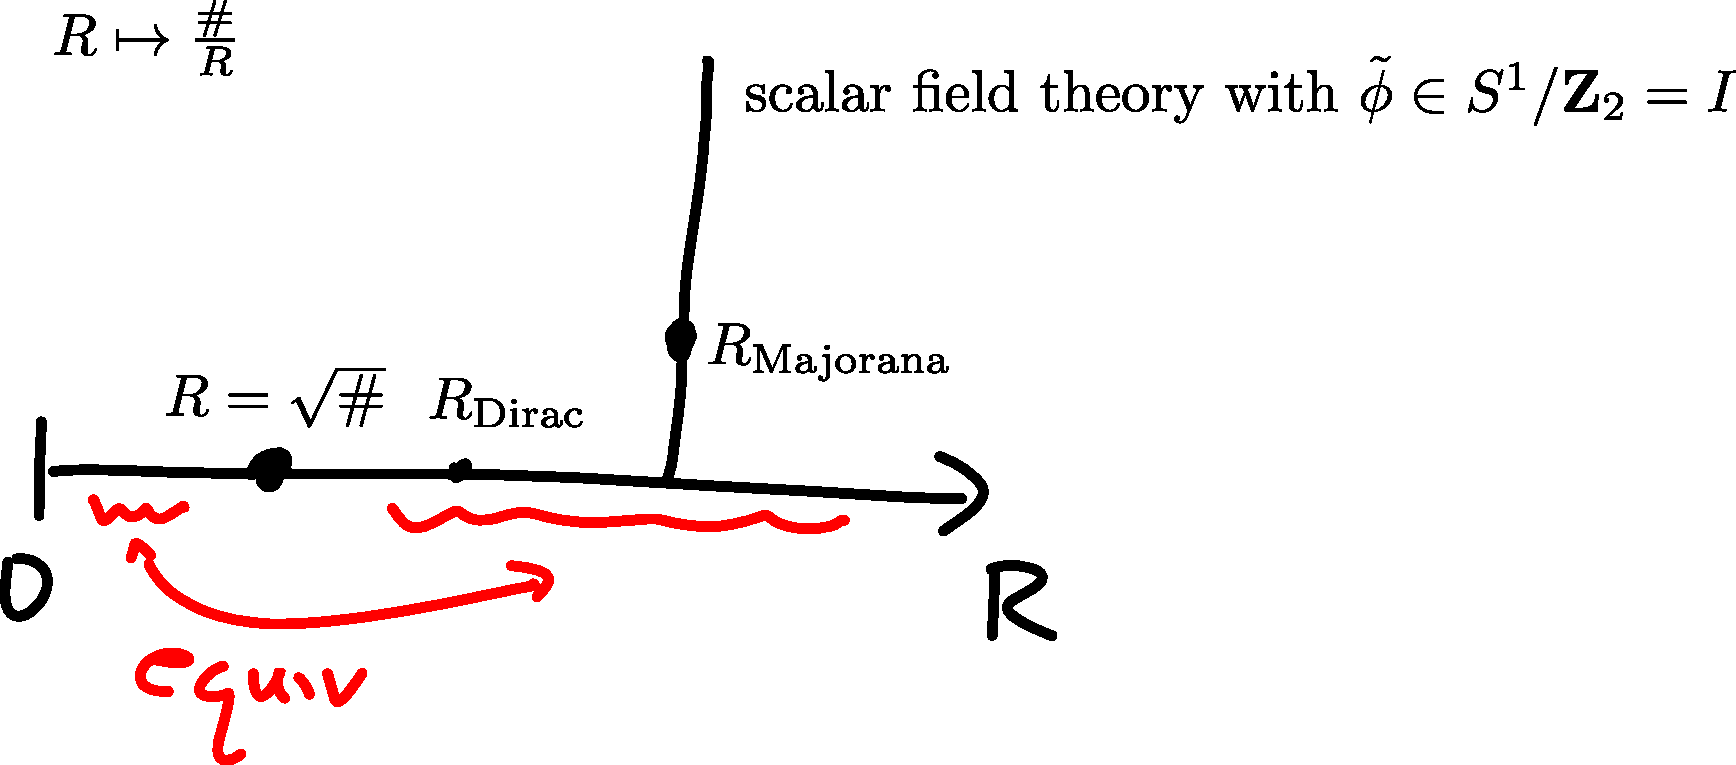
\includegraphics[width = 7in]{fig/lecture3CFTchart.pdf}
\end{center}





